\section{Source Localisation using TDoA}

The two main aspects of being able to localise GWs in this experiment are the detector analogues and the localisation methods. The detector is able to take the video data from the webcam and convert it into an incident time by looking at when the displacement of the physical water detector is above a certain threshold. The localisation methods deploy two separate methods, one being the triangulation method and the other being the minimising of an objective function to remove degeneracy in the triangulation results.

\subsection{Detector Output}
\label{sec:4.1.1}
Determining the time at which the wave arrives at the detector, yields TDoA times which can be used to localise the source. Once positional data is gathered from the detection of the motion of an object on water using a trained ML algorithm to accurately map such movement, this data can give the time differences necessary for this experiment. As mentioned in Section \ref{sec:3.4}, a JSON file is used to store the $x,y$ coordinates of the bob, these coordinates are no use on their own so must be reduced into one dimension to be able to visualise the detection of the wave. Applying Pythagoras' we are able to gather the distance moved by the object per instance (in this case per frame recorded). Where the displacement of the object between two consecutive frames $a$ and $b$ is 
\begin{equation}
    displacement = \sqrt{(x_b-x_a)^2+(y_b-y_a)^2}.
\end{equation}
 As the camera records at 30 FPS we know that the time between each frame is then 1/30s therefore we can plot displacement as a function of time. For three detectors we gather three separate readings of the detected wave. The motion of the object is expected to produce a large initial peak which gradually reduces over time as it oscillates, much like a lightly damped pendulum, as each successive wavefront carries less energy than its predecessor. In reality this is not the case and instead the motion is massively dampened and brought back to its original state in a matter of 
\begin{figure}[h!]
    \centering
    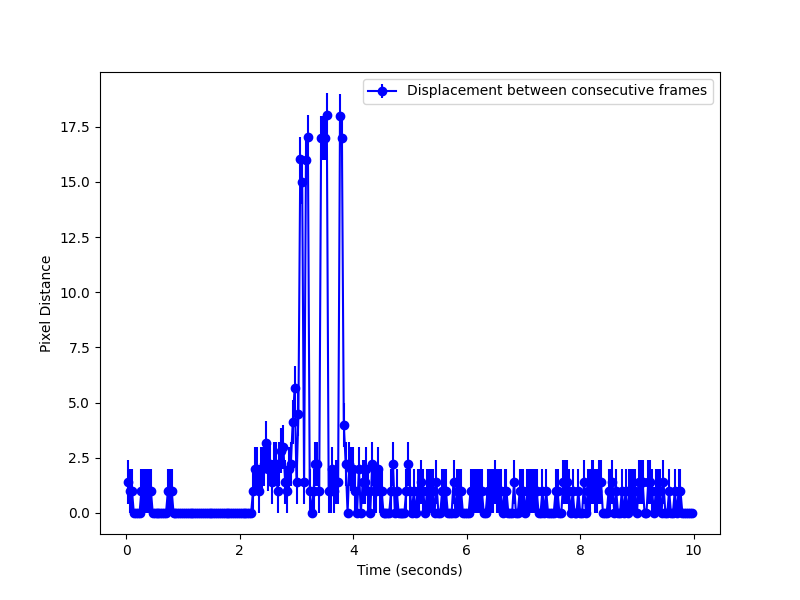
\includegraphics[width=0.6\linewidth]{images/d1.png}
    \caption{Distance travelled by the bob between successive frames as measured from detector 1.}
    \label{fig:d1}
\end{figure}

\begin{figure}[h!]
    \centering
    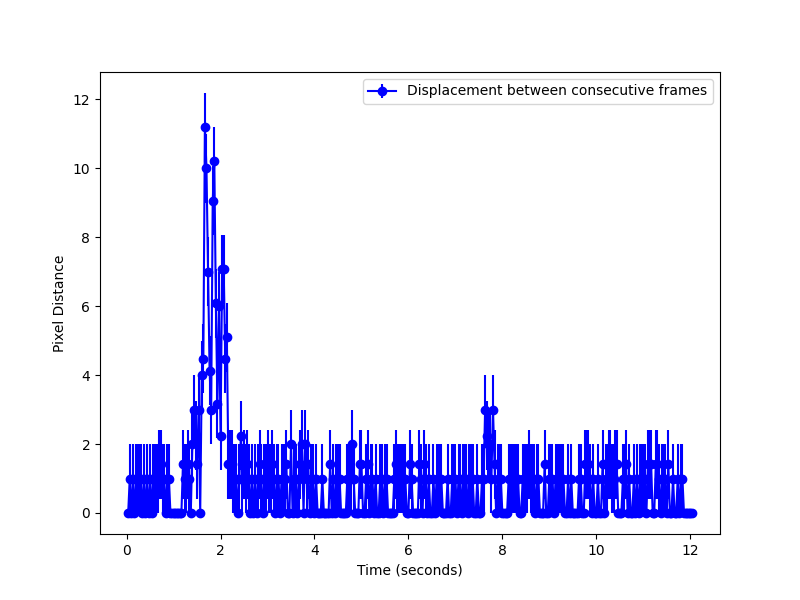
\includegraphics[width=0.6\linewidth]{images/d2.png}
    \caption{Distance travelled by the bob between successive frames as measured from detector 2.}
    \label{fig:d2}
\end{figure}

\begin{figure}[h!]
    \centering
    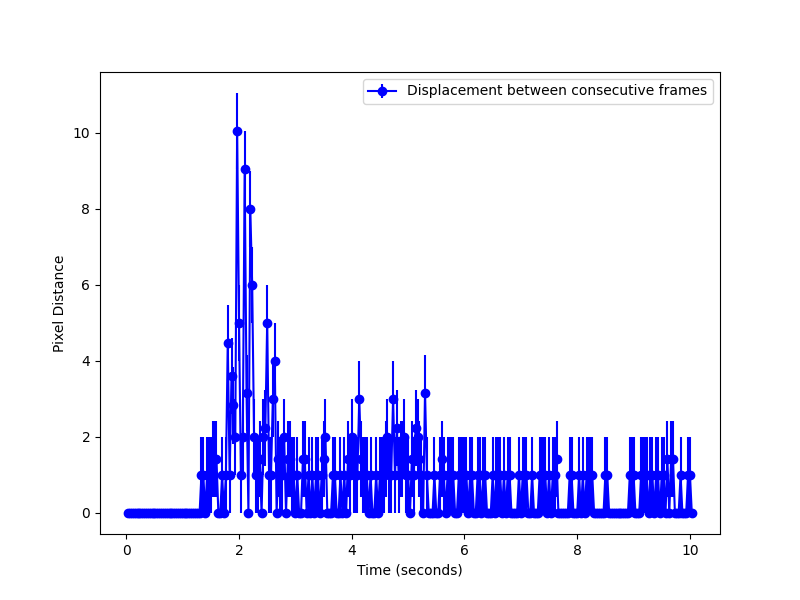
\includegraphics[width=0.6\linewidth]{images/d3.png}
    \caption{Distance travelled by the bob between successive frames as measured from detector 3.}
    \label{fig:d3}
\end{figure}


False positives can occur from this as there may be instances where one detector observes an event at a certain time point. Upon checking other sensors it becomes apparent that no GW had occurred as other detectors would have also observed a similar wave but shifted in time as a result of the difference in distances between the source and multiple detectors. These false positives may happen due to seismic activity in GW detectors, or in our case simply knocking one of the detectors can cause this. A small perturbation in Figure \ref{fig:d2} at roughly $t = 8 \space s$ may be caused by the detector being knocked slightly as it does not show up on any of the other observed measurements.

In all three figures there is an associated uncertainty of $\pm 1\space pixel$ as the bounding box is one pixel thick and the position of the object is taken as the centre of the bounding box thus approximated by these finite-sized pixels. As the true position can lie anywhere within a pixel, but the sensor can only record it as being at the centre of that pixel.

Once all three readings from the detectors have been gathered the time at which each sensor detected the wave can be gathered, $t_i,\space i \space\in \space [1,2,3]$. Since in each graph there is a ramp-up time so to speak where the bob slowly moves with the initial wavefront before reaching its maximum displacement there are uncertainties as to when the wave initially interacts with the bob. This ramp-up period can be attributed to the overall responsiveness of the detector depending on wave speed, inertia and damping effects. Such as the fact that the bob was not freely suspended and was making contact to the walls of the glass tube, therefore friction had to be overcome. To measure $t_i$ we take the time at which the bobs displacement is above a certain threshold and introduce an uncertainty relative to the sampling rate of the camera where a higher FPS can reduce time discretisation errors. We estimate the uncertainty of $t_i$ to be $\pm2$ frames or $\pm0.07s$ for a 30 FPS sampling rate.

\subsection{Triangulation Results}

Upon obtaining values for $t_i$ we plug these times into Equations \ref{eqn:dd_12} and \ref{eqn:2.2} along with the measured velocity mentioned in Section \ref{sec:ML-training}. Along with the known positions of the detectors we are able to minimise Equation \ref{eqn:SF} and plot Equations \ref{eqn:dd12}, \ref{eqn:dd13} and \ref{eqn:dd12} in order to verify the location of the source. We developed a python script in order to aid in this as minimising the source function is a computationally intensive task \cite{boxer_2025_15041819}. 

Using the triangulation method by solving three hyperbolic equations we are able to retrieve the location of the source. Figure \ref{fig:triangulation} utilises this method showing overlapping hyperbolic functions at a singular position. As discussed in Section \ref{sec:hyp-ass} a degeneracy can occur in some instances where the source is located closer to the edge of the box than the centre. Instead of introducing a fourth sensor we are in fact able to localise the source by minimising the source function which aids in the localisation in Figure \ref{fig:triangulation}. 

\begin{figure}
    \centering
    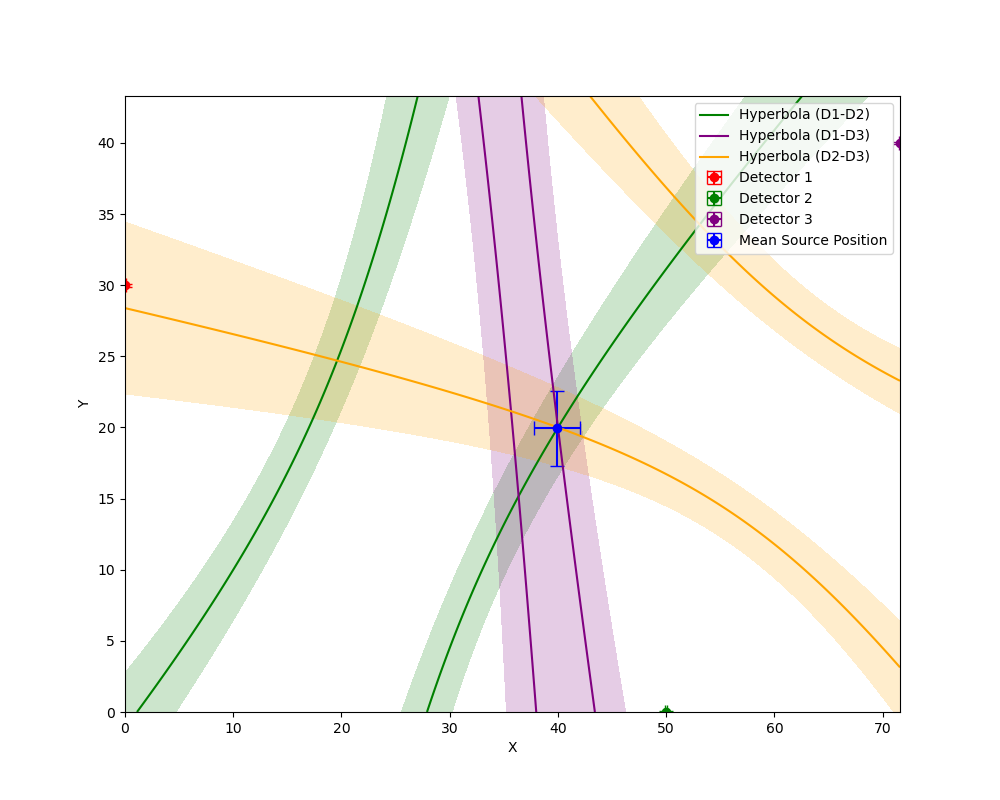
\includegraphics[width=0.75\linewidth]{images/triangulator.png}
    \caption{Triangulation of the source position using hyperbolic functions.}
    \label{fig:triangulation}
\end{figure}

In this instance of determining the location of the source through intersecting hyperbolas, due to assuming Gaussian uncertainties and the shape of the hyperbolas the area in which the source could be is restricted by the shaded area where all three uncertainties intersect. We can accurately depict the shape of the uncertainty area in which the source lies through sampling the position through normalised random uncertainties i.e. the Monte Carlo method \cite{boxer_2025_15041819}. 

\section{Monte Carlo Simulation}

The Monte Carlo method is used to map the uncertainty in the source position by sampling from the distributions of the input parameters (arrival times, detector positions, and wave speed). For each sample, the source position is estimated by minimising the source function, Equation \ref{eqn:SF}. The mean and standard deviation of the sampled source positions provide an estimate of the source position and its uncertainty. The minimisation is performed using the \lstinline{scipy.optimize.minimize} function. The following steps are performed in the Monte Carlo simulation:
\begin{enumerate}
    \item Sample arrival times, detector positions, and wave speed from their respective distributions.
    \item Calculate the distance differences \(\Delta d_{12}\) and \(\Delta d_{13}\) for each sample. 
    \item Estimate the source position by minimising the distance difference function.
    \item Repeat the process for a large number of samples (e.g., 1000) to build a distribution of source positions.
\end{enumerate}

Once all the steps have been carried out we can plot the sampled locations as a 2D histogram mapping the probability distribution of the source position where brighter regions indicate a higher confidence in the source location, Figure \ref{fig:hist}. Two 1D histograms are included on the $x$ and $y$ axis which simply plot the distribution in their respective coordinates, fitted with a Gaussian curve to confirm that errors are normally distributed and gives us a simple $\mu \space\pm\sigma$ uncertainty estimate. The plot includes $1\sigma$ and $2\sigma$ contour lines to mark the probability regions i.e. there is a $68.3\%$ chance the true position lies within the $1\sigma$ contour. These contour lines help quantify the uncertainty in the location and show how errors affect the mean position. 

\begin{figure}[h!]
    \centering
    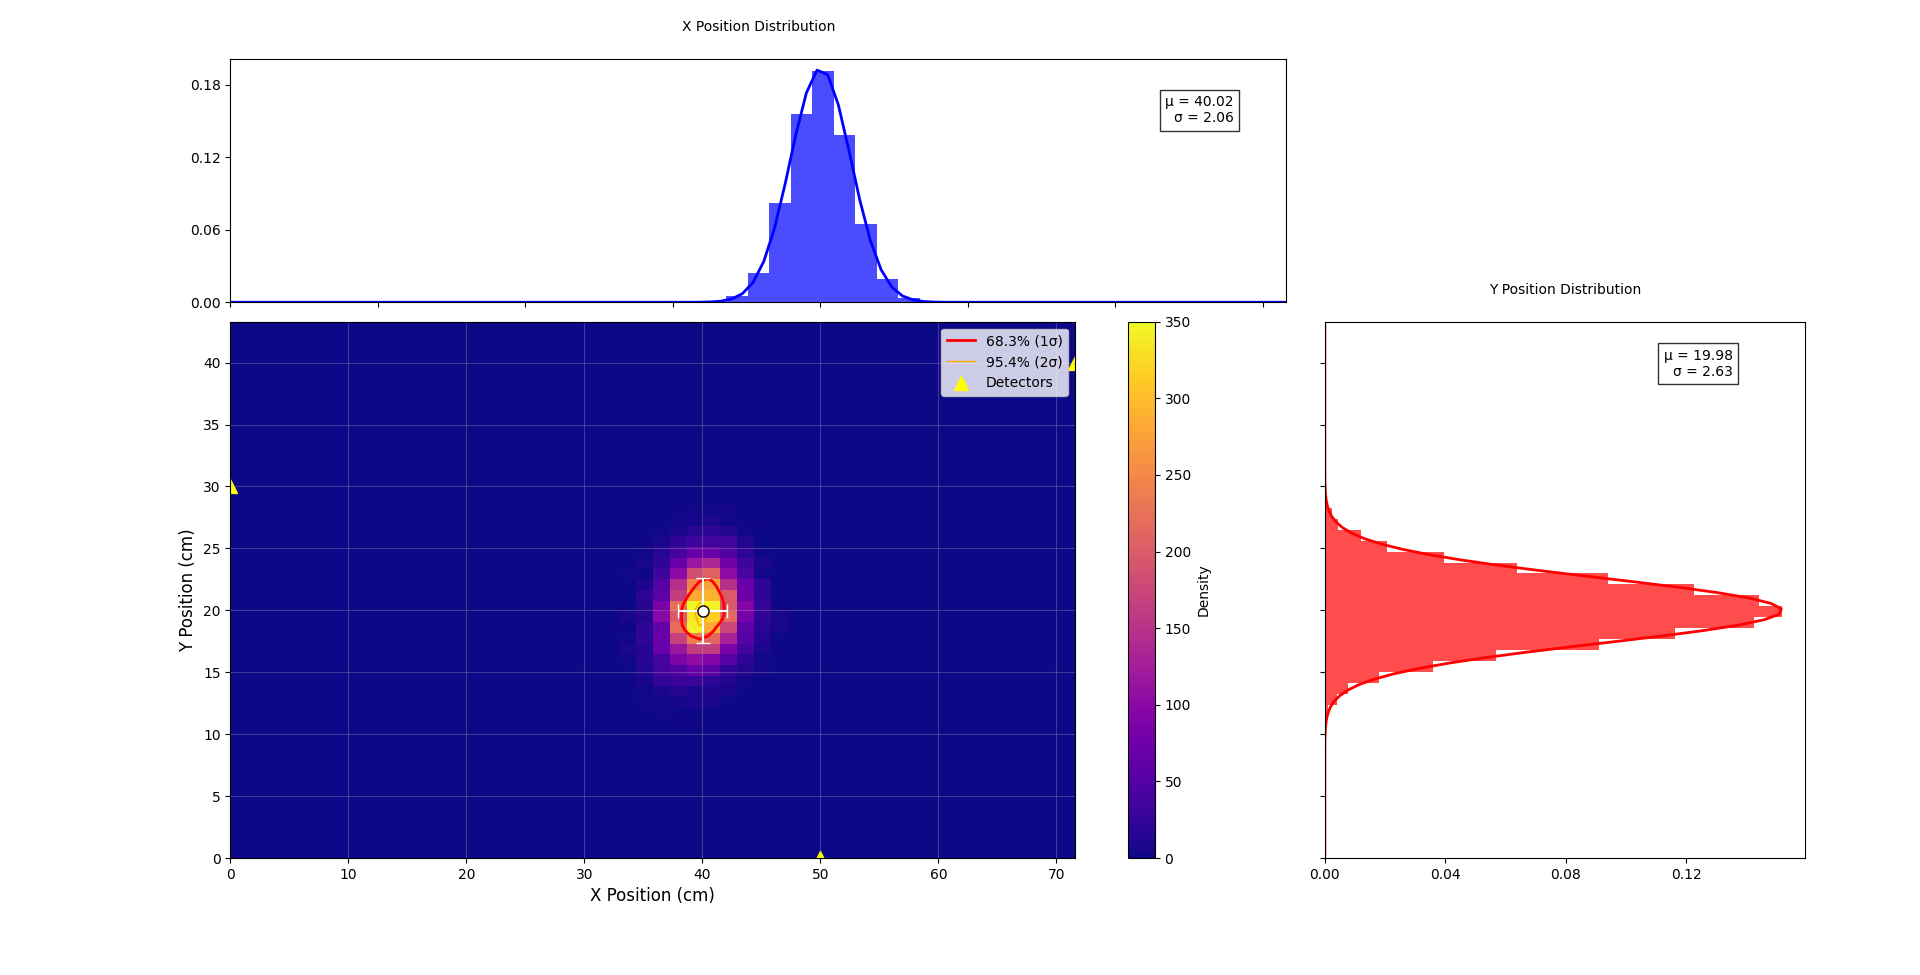
\includegraphics[width=1\linewidth]{images/hist.png}
    \caption{Source position from TDoA measurements. The 2D density plot (centre) shows the probability distribution of the source location, with red $(68.3\%, 1\sigma)$ and orange $(95.4\%, 2\sigma)$ contours marking confidence regions. 1D histograms (top/right) display projected uncertainties along each axis, with Gaussian fits (blue/red curves) indicating normally distributed errors. The white circle marks the mean position. Detector geometry and timing uncertainties propagate into the observed asymmetric confidence regions.}
    \label{fig:hist}
\end{figure}

We can show how increasing and decreasing the uncertainty in the velocity can change the uncertainty region in Figure \ref{fig:unc-change}, for example. Figure \ref{fig:det-01dv} shows how a greatly reduced uncertainty in the velocity can affect the shape of the contour lines and therefore the overall shape of the confidence region in which the source lies, Figure \ref{fig:det-01dv} does not seem to differ that far from Figure \ref{fig:hist} in terms of the shape of the contour lines or the uncertainty region, one could conclude that this measurement is not a dominant factor in the overall uncertainty of the source position. When blown up to $50$ times its measured value Figure \ref{fig:50dv} shows how the shape of the confidence region changes based on a large change in uncertainty. This change in shape by the uncertainty region shows a possible flaw in the detector network where along direction in the plane it is more susceptible to perturbations in uncertainties due to the arrangement of the detectors a weakly constrained direction in the plane will be present. To mitigate this it can prove useful to add an extra detector to break any degeneracies that may arise and constrain the uncertainty region.

\begin{figure}[h!]
    \centering
    \begin{subfigure}[b]{.47\textwidth}
      \centering
      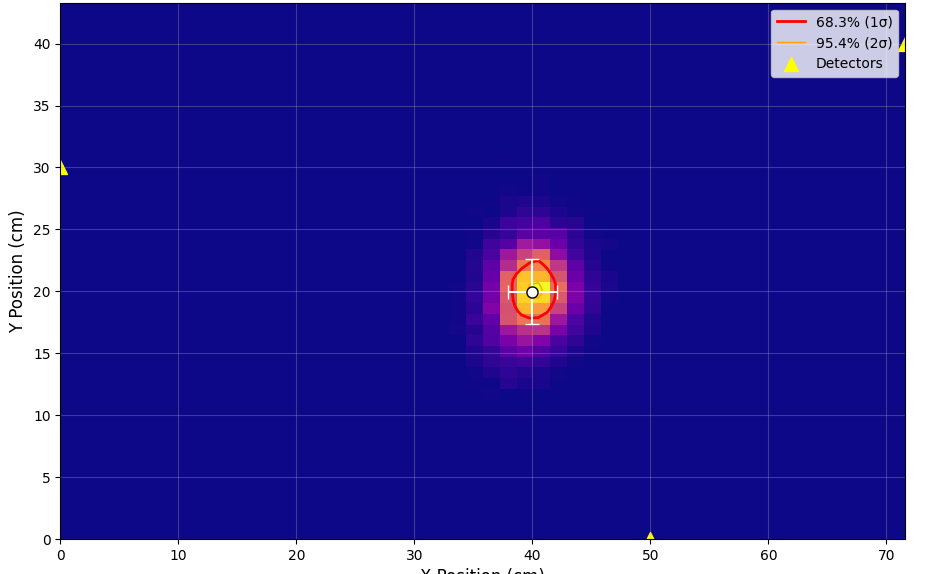
\includegraphics[width=\textwidth]{images/01dv.png}
      \caption{}
      \label{fig:50dv}
    \end{subfigure}%
    \begin{subfigure}[b]{.53\textwidth}
      \centering
      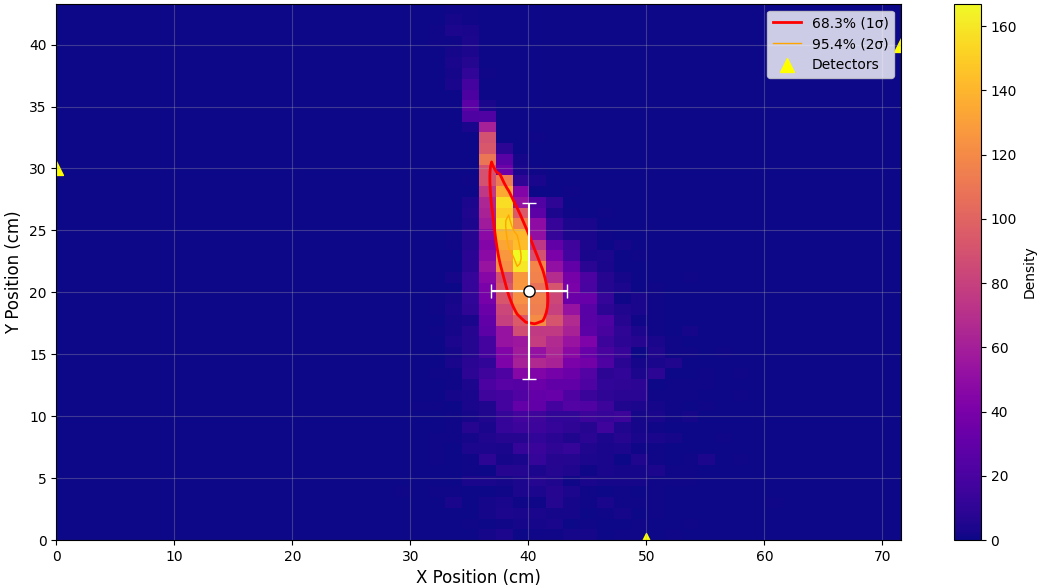
\includegraphics[width=\textwidth]{images/50dv.png}
      \caption{}
      \label{fig:det-01dv}
    \end{subfigure}
    \caption{(\textbf{a}) 2D density plot shows how a very small uncertainty in the velocity measurement can affect the shape of the uncertainty region, with contours marking confidence regions and outlining the shape of said region. (\textbf{b}) 2D density plot shows how a large uncertainty in the velocity measurement can affect the shape of the uncertainty region, with contours marking confidence regions and outlining the shape of said region. Exposing the weaknesses with the three detector system in which an weakly constrained direction appears within the uncertainty region.}
    \label{fig:unc-change}
\end{figure}

\section{Comparison with Gravitational Wave Signals}

\begin{figure}[h!]
    \centering
    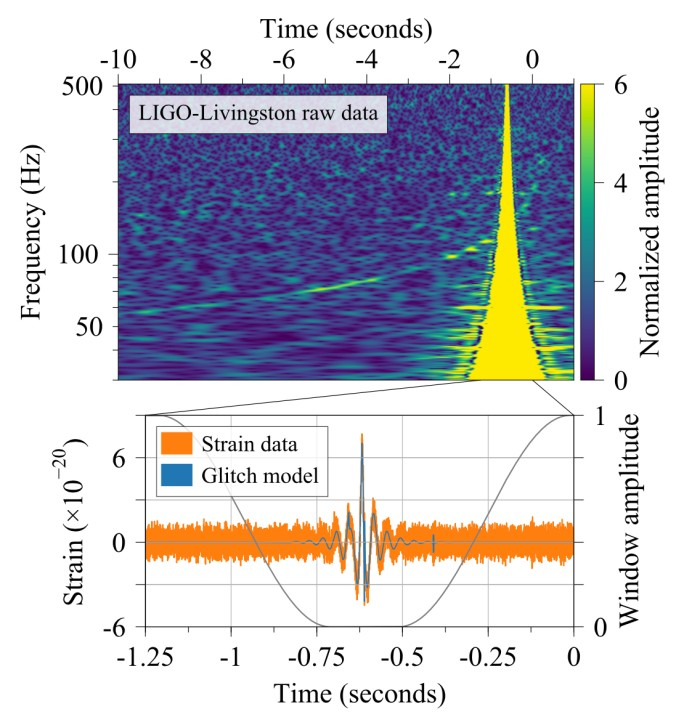
\includegraphics[width=0.5\linewidth]{images/ezgif-2cd7de674685b7.jpg}
    \caption{GW170817 signal detected by the LIGO-Livingston detector. Top panel depicts the time-frequency detection of the GW. Bottom pannel depicts the raw strain data measured by the detector, the shape of which being an indicator to the type of source. \cite{Abbott_2017}}
    \label{fig:NS-GW}
\end{figure}


The signal observed in our water wave detectors (Figures \ref{fig:d1}, \ref{fig:d2}, and \ref{fig:d3}) exhibits a rapid rise in displacement followed by a gradual decay, which is qualitatively similar to the expected behaviour of a GW signal. However, the ``ring-down" phase, where the detector continues to oscillate as the wave passes, is significantly damped in the experiment due to friction between the bob and the walls of the glass tube, as well as viscous damping in the water. In real GW detectors like LIGO, the signal from a merging binary neutron star system shows a characteristic "chirp" pattern, where the frequency and amplitude increase as the objects spiral inward before merging, followed by a damped sinusoidal ring-down (Figure \ref{fig:NS-GW}).



